\section{Framework}
\label{sec:framework}

\subsection{Overview}
\label{sec:framework_overview}

The framework constructs paired network and corridor distributions for each
country-service group. It combines traceroute, probe metadata, IP geolocation
and ASN mappings, AS context, and cable metadata. Figure
~\ref{fig:framework_pipeline} shows the three components in processing order:
path extraction creates atomic hop-pair segments, corridor projection
constructs each segment's feasible landing-region corridor set, and
aggregation forms the paired distributions. Complete traceroutes supply the
exposure denominator.

The outputs retain the distinction between trace-level exposure and
segment-level distributions. Exposure records whether a path contains at
least one inter-region feasible corridor. The distributions condition on
candidate-bearing observations and compare how their mass is organized across
logical transitions and physical directions.

\begin{figure*}[t]
\centerline{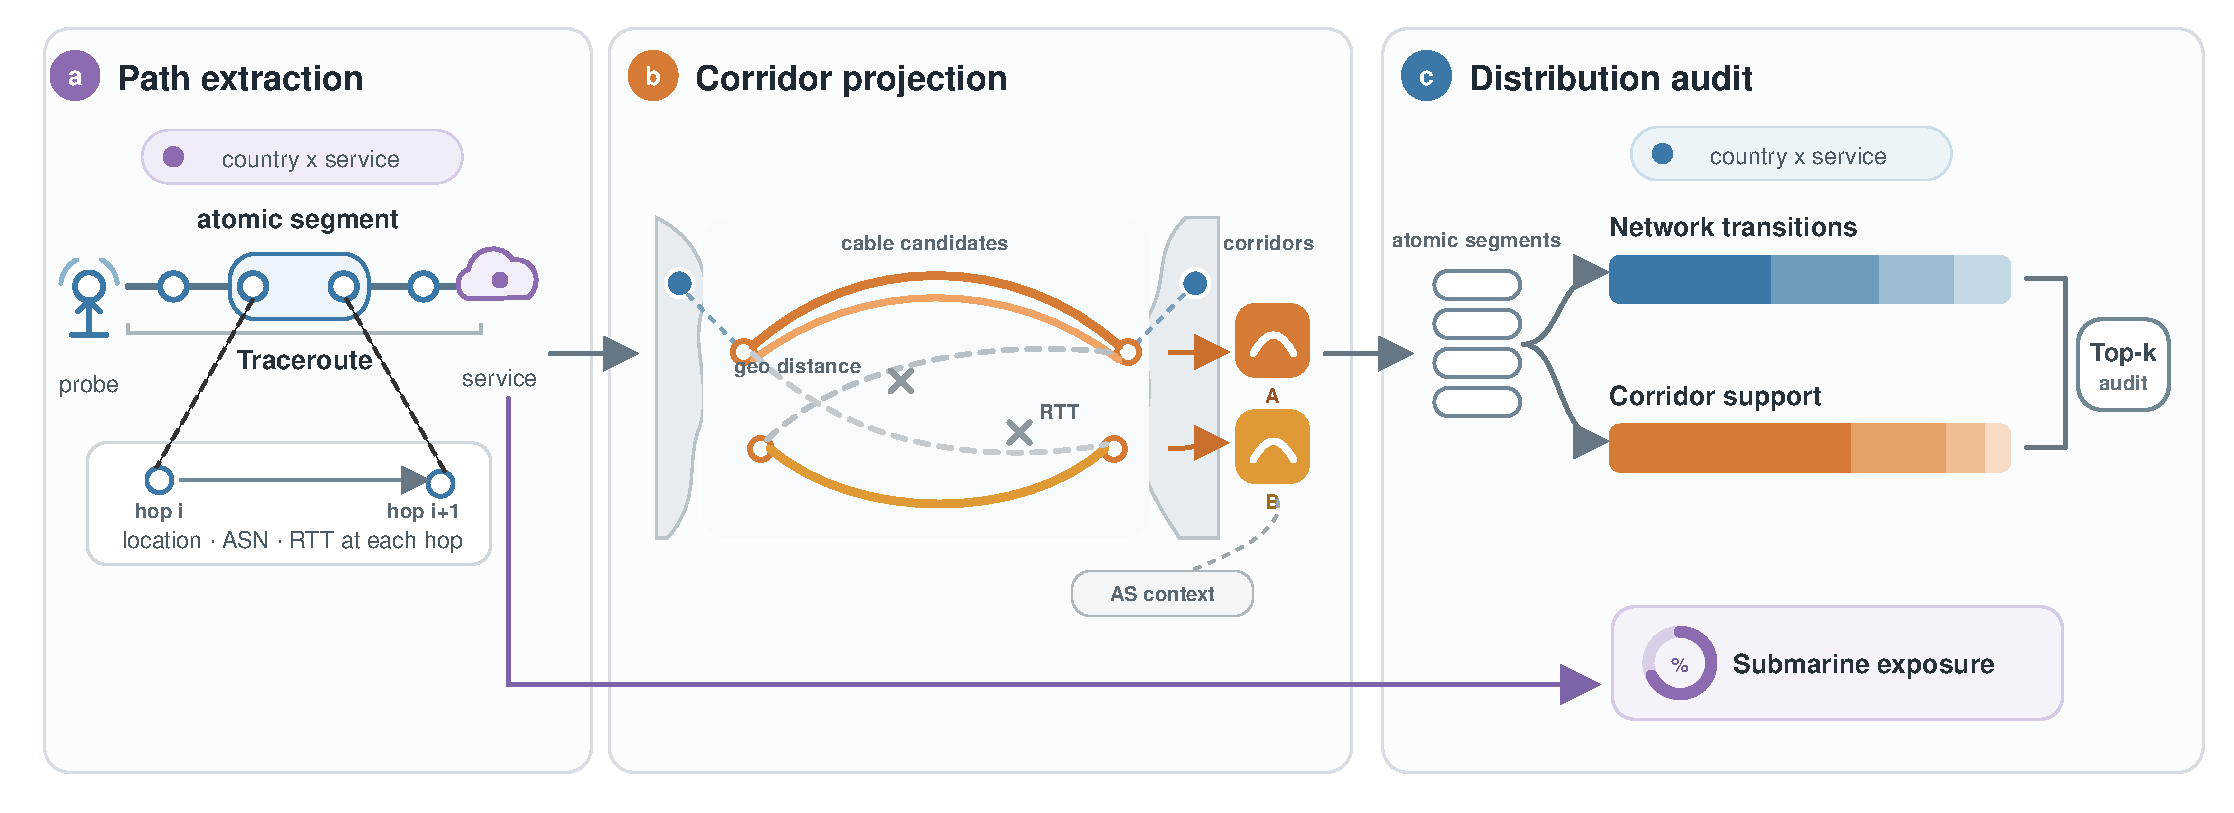
\includegraphics[width=\textwidth]{figures/framework_cross_layer_audit.pdf}}
\caption{Cross-layer audit framework.}
\label{fig:framework_pipeline}
\end{figure*}

\subsection{Path Extraction}
\label{sec:framework_path_segmentation}

We group traceroutes by probe country and measured service to retain the
source-side connectivity context and deployment-specific destination
selection. Hop countries remain segment attributes.

We normalize each traceroute into visible hops with locations, ASNs, and RTTs.
The analysis uses the complete visible sequence. An auxiliary path-entry view
ends at the first appearance of the target ASN.

Successive visible, geolocated hops form atomic segments. Each segment records
endpoint locations, ASNs, countries, positions, RTT difference, and bridged-hop
count. Repeated hops and RTT samples retain their trace identity and ordering.
When timeouts separate two visible hops, the bridged-hop count records the gap
for pipeline accounting.

When both endpoint ASNs are available, their ordered pair is the segment's
network-transition label. Segments with one missing endpoint ASN receive an
ordered country-pair fallback label.

Audit eligibility is evaluated over the complete country-service group. It
requires a country-fallback share of at most 30\%, at least 30
candidate-bearing segments, 10 probes, and 3 probe ASNs.

\subsection{Corridor Projection}
\label{sec:framework_projection}

\paragraph{Landing-station and cable candidates.}
Landing stations within 50~km of each endpoint are paired through cable systems
active on July~1, 2026. Explicit path or branch information defines direct
cable segments; unordered landing-point membership defines reachability at the
metadata's topology resolution and is recorded in provenance.

Endpoint catchment retrieves landing stations, and landing-region grouping
organizes them into coastal regions. The 50-km catchment retrieves stations
consistent with router geolocation; the 30-km diameter groups the retrieved
stations. Cable lifecycle filtering is applied before region pairs are formed.

\paragraph{Geographic and delay feasibility.}
Let \(D\) be the great-circle distance between a candidate landing pair and
\(v_f=200\)~km/ms the effective propagation speed in fiber. A candidate is
propagation-feasible when

\begin{equation}
    \Delta RTT + \tau \geq \frac{2D}{v_f},
    \label{eq:rtt-feasibility}
\end{equation}

where \(\Delta RTT\) is the segment RTT difference and \(\tau=5\)~ms. For
non-positive or inconclusive differences, candidates use the geographic and
lifecycle constraints and retain an RTT-status flag.

The inequality compares the observed round-trip increment with the minimum
round-trip propagation time between landing points. It operates as a feasibility
condition alongside endpoint proximity and cable connectivity.

\paragraph{Diameter-limited landing regions.}
Landing stations are grouped into regions with a 30-km maximum pairwise
distance. A \emph{landing-region corridor} is a direction-independent region
pair connected by a feasible cable candidate. Multiple cables and exact landing
pairs may contribute to one corridor; distinct coastal entry-exit patterns
remain separate.

The aggregate distribution uses the complete feasible corridor set, with the
corridor as its primary physical unit. Cable candidates and exact landing
pairs remain linked in the outputs. A supplementary ranking uses landing
proximity, propagation consistency, and AS context.

\paragraph{Observation mass.}
Duplicate cable rows belonging to the same corridor are collapsed within each
atomic segment. For a segment (s) with feasible corridor set
\(\mathcal{C}_s\), the corridor mass is

\begin{equation}
    w_{s,c}=\frac{1}{|\mathcal{C}_s|},
    \qquad c\in\mathcal{C}_s.
    \label{eq:uniform-mass}
\end{equation}

Thus \(\sum_{c\in\mathcal{C}_s} w_{s,c}=1\): each candidate-bearing segment
contributes equal total observation mass, distributed according to candidate
multiplicity.

\subsection{Measurement Configuration}
\label{sec:framework_configuration}

Table~\ref{tab:measurement-configuration} lists the common configuration.

\begin{table}[!t]
  \centering
  \caption{Cross-layer measurement configuration.}
  \label{tab:measurement-configuration}
  \footnotesize
  \setlength{\tabcolsep}{3.6pt}
  \begin{tabular}{lr}
    \toprule
    Parameter & Value \\
    \midrule
    Endpoint landing catchment radius & 50 km \\
    Landing-region maximum diameter & 30 km \\
    Fiber propagation speed & 200 km/ms \\
    RTT tolerance & 5 ms \\
    Same-city threshold & 25 km \\
    Cable lifecycle & Active on July 1, 2026 \\
    Inconclusive RTT & Retained and flagged \\
    Timeout-bridged segment & Retained and flagged \\
    Primary path scope & Complete visible sequence \\
    \bottomrule
  \end{tabular}
\end{table}

\subsection{Physical Mapping Resolution}
\label{sec:framework_mapping_resolution}

Table~\ref{tab:mapping-resolution} classifies each segment by input coverage and
the size of \(\mathcal{C}_s\).

\begin{table}[!t]
  \centering
  \caption{Segment-level physical mapping resolution.}
  \label{tab:mapping-resolution}
  \footnotesize
  \setlength{\tabcolsep}{3.2pt}
  \begin{tabular}{p{0.30\columnwidth}p{0.60\columnwidth}}
    \toprule
    State & Operational definition \\
    \midrule
    Single corridor
      & Feasibility inputs available and \(|\mathcal{C}_s|=1\) \\
    Bounded multi-corridor
      & Feasibility inputs available and \(|\mathcal{C}_s|>1\) \\
    No feasible corridor
      & Feasibility inputs available and \(|\mathcal{C}_s|=0\) \\
    Insufficiently resolved
      & Insufficient location, path-visibility, or metadata fields for stable
        corridor construction \\
    \bottomrule
  \end{tabular}
\end{table}

Single- and bounded multi-corridor segments form the physical distribution.
Pipeline accounting retains the other states, and all valid traces form the
exposure denominator.

Candidate-set size and aggregate concentration describe different levels of
the analysis. A unit may contain many bounded segments yet concentrate after
their uniformly allocated mass repeatedly supports the same corridors.

\subsection{Distribution Aggregation}
\label{sec:framework_distribution_analysis}

For each probe-country and service group, we construct both distributions
from candidate-bearing atomic segments. Counting ordered endpoint-AS labels
gives the network-transition probabilities \(p^{N}\). Summing the corridor
masses in Eq.~\eqref{eq:uniform-mass} and normalizing within the group gives
the corridor probabilities \(p^{C}\).

For each auditable country--measurement unit \(u\), let \(S_u\) denote the
candidate-bearing atomic segments and \(\ell(s)\) the label assigned to
segment \(s\). Each distinct segment contributes once to an ordered
network-side label at its available mapping resolution. The probability of
label \(t\) is

\[
p_u^{N}(t)=
\frac{\sum_{s\in S_u}\mathbf{1}[\ell(s)=t]}
{|S_u|}.
\]

Direction is preserved throughout the aggregation. We summarize the
distribution using its Top-2 share, defined as the combined probability
of the two most frequent network-side labels. Higher values indicate
that the observed network-side structure is concentrated in fewer
dominant labels.

Submarine exposure uses complete valid traceroutes. A traceroute is exposed
when at least one segment has a feasible inter-region corridor. Dividing the
exposed-trace count by all valid traces in the country-service unit gives the
exposure rate.

Three metrics summarize each distribution. Top-2 share is the sum of the two
largest probabilities. The effective category count is
\(\exp[-\sum_i p_i\log p_i]\) and measures breadth on the scale of an equally
weighted category count. Normalized entropy divides Shannon entropy by log
support size. Network-to-corridor differences are computed within each unit.

The metrics distinguish dominant-corridor mass from the long tail and support
size. Top-2 share emphasizes leading categories, effective count incorporates
the complete probability vector, and normalized entropy measures evenness
relative to observed support.

A common 80\% Top-2 threshold supplies four descriptive classes: broad at both
layers, concentrated at both, network-broad/corridor-concentrated, and the
reverse. Continuous Top-2 shifts, effective counts, and normalized entropy
accompany the classification.
